% meaty.tex — fixture exercising the RRP-0015 meaty-claim fields.
%
% One claim with a paired evidence block. The evidence block contains a
% figure input and a few \dependson lines; the parser must:
%   - capture the proof body into Claim.proof (with math + paragraph
%     breaks preserved and the \dependson lines stripped),
%   - capture the % fig-meaty.tex — placeholder figure for the meaty-fixture.
\begin{figure}[H]
\centering
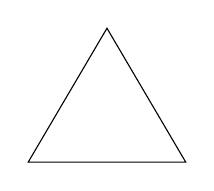
\begin{tikzpicture}
  \draw (0,0) -- (2,0) -- (1, 1.7) -- cycle;
\end{tikzpicture}
\caption{The equilateral triangle $ABC$ constructed on $AB$.}
\label{fig:meaty}
\end{figure}
 reference into
%     Claim.figures[],
%   - populate Claim.source_location.{file,line_start,line_end} from
%     the claim/evidence span.
%
% A second claim with no paired evidence exercises the "no proof
% attached" branch.

\documentclass{rrxiv}

\rrxivid{rrxiv-meaty-fixture}
\rrxivversion{v1}
\rrxivprotocolversion{0.2.0}
\rrxivlicense{CC-BY-4.0}

\title{Meaty-claim fixture}
\author{rrxiv Project}

\begin{document}
\maketitle

\begin{abstract}
A parser-conformance fixture for the RRP-0015 meaty-claim fields.
\end{abstract}

\section{Constructions}
\label{sec:constructions}

\begin{claim}[Proposition I.1: Equilateral triangle]
\label{prop:I.1}
On a given finite straight line to construct an equilateral triangle.
\end{claim}

\begin{evidence}[Proof of I.1]
\label{ev:I.1}
% fig-meaty.tex — placeholder figure for the meaty-fixture.
\begin{figure}[H]
\centering
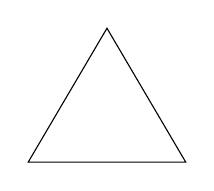
\begin{tikzpicture}
  \draw (0,0) -- (2,0) -- (1, 1.7) -- cycle;
\end{tikzpicture}
\caption{The equilateral triangle $ABC$ constructed on $AB$.}
\label{fig:meaty}
\end{figure}

Let $AB$ be the given finite straight line. With centre $A$ and
distance $AB$ describe the circle $BCD$.

By Common Notion 1, $AC = BC$. Therefore the triangle $ABC$ is
equilateral.
\dependson{I.1}{post:1}
\dependson{I.1}{post:3}
\end{evidence}

\begin{claim}[Definition: a point has no part]
\label{def:I.1}
A point is that which has no part.
\end{claim}

\end{document}
